\chapter{Dark Horse}

在本学期新开始的dark horse阶段,我们提出了如下两个设计方向供考究。

\begin{itemize}
\item 教学楼内的教学辅助机器人
\item 图书馆里的书籍整理机器人
\end{itemize}

具体的方案如下:

\section{教学楼内的教学辅助机器人}

利用机器人的远程呈现的功能,在多媒体教学设备出现问题时,可以远程的实时
的进行辅助修理,或者远程的实现教学内容的采集与反馈。

\section{图书馆里的书籍整理机器人}

新图书馆采用的电子标签为RFID标签,与此相关,在机器人上加装RFID(如下图)
标签探测,对书架进行循环检测,如果有放错书籍的情况出现,可以远程的反馈
信息。如此来解决许多书本因为放错位置而难以找寻的问题。

\begin{figure}[h]
        \centering
                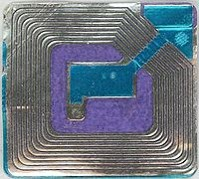
\includegraphics[width=.70\textwidth]{Figures/ch6.rfid.jpg}
        \caption{RFID}
        \label{fig:rfid}
\end{figure}

对于以上的设计方向,我们在第三教学楼和图书馆中进行了相应的采访、问卷等
方式的具体调查,分析结果如下:

教学设备辅助使用,问题多出现于学期初,且目前突发问题的处理速度并不很慢,
所以实现此用途看来并不合理。教学视频的动态录制,不拘泥于单一的旋转摄像
头的视角,以机器人的灵活视角来捕捉课堂信息,并可通过网络广播。如此一来,
机器人所具备的优势就仅限于自由移动方面,而且考虑到教室的空间自由问题,
这一提议并不十分可行。

图书馆书籍整理,询问了相关图书馆的书籍整理人员,得到的反馈是,这一类问
题是可以被人力来较好的解决的,而且随着技术熟练度的提高,目前已经不是很
大的问题。单纯利用机器人,效率问题难以解决。

最后,在李卫平院长的提议下,我们把最终的目标定位为一个部门、机构专用的
远程虚拟出席设备,利用机器人的灵活移动的特性,能够较好的实现远程现场情
况的采集。

我们的主要任务定位为,将这一功能的实现做的尽量的实用、高效。
